\documentclass[10pt,conference,compsocconf]{IEEEtran}

\usepackage{hyperref}
\usepackage{graphicx}	% For figure environment

% Packages added by Joachim

%drow graph
\usepackage{fancybox}
\usepackage{tikz}
\usepackage{capt-of}
\usepackage{verbatim}

% cancel math expression
\usepackage{cancel}

% math
\usepackage{amsmath}


\begin{document}
\title{PCML CS-433: Higgs Challenge Project}

\author{
  Joachim Muth, SCIPER 214757, joachim.muth@epfl.ch\\
  Junze Bao, SCIPER 266983, junze.bao@epfl.ch\\
  Chanhee Hwang, SCIPER 260872, chanhee.hwang@epfl.ch\\ \\
  \textit{School of Computer and Communication Sciences, EPF Lausanne, Switzerland}
}

\maketitle

%========================
\begin{abstract}
...
\end{abstract}

%========================
\section{Introduction}
The ATLAS experiment consists of collisions between protons. Particles created by these collisions are detected by sensors, producing a sparse vector of about a hundred thousand dimensions. Analyzing these data, ATLAS team try to estimate if the detected particles comes from a Higgs boson decay.

The \emph{Higgs boson machine learning challenge} consists of a large dataset of particles decay detections labeled as Higgs or background. The dataset is composed of thirty features and is already cleaned from a lot of well-known background effect well-known by the ATLAS team. Also, in order to balance the great number of background events compared to Higgs events, the size of both dataset is balanced.~\cite{higgsChallenge}

%========================
\section{Models and Methods}

\subsection{Split of the data}
In order to chose which features to keep in the machine learning modelling we did, and to deal with the great number of \emph{NaN} in the data set, we analyzed their distrubution. 

It show that it's possible to cathegorize the events into four different sets based on the number of jets (\emph{int} $\in [0, 3]$). There is a physics reason behind it, since some measures make no sens for some jet numbers. \cite{higgsChallenge}.

Once this split proceeded, subsets share all the same defined features, except the estimated mass $m_H$ of the Higgs boson candidate. Once again, these subsets are split into two subsets to obtain, finally, eight different subsets to model (see figure \ref{split})

\begin{figure}[tbp] %-------TIKZ PICTURE---------
  \centering
  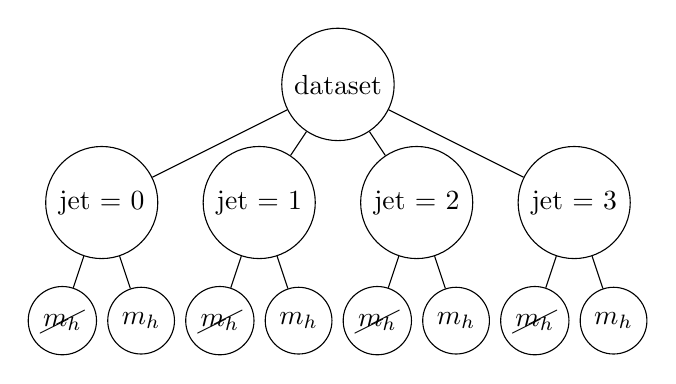
\begin{tikzpicture}[level/.style={sibling distance=20mm/#1}]
  \node [circle,draw] (z){dataset}
  child {node [circle,draw] (a) {jet = 0}
    	child {node [circle,draw] (b) {$\cancel{m_h}$}
    	}
  	child {node [circle,draw] (g) {$m_h$}
  	}
  }
  child {node [circle,draw] (j) {jet = 1}
      	child {node [circle,draw] (b) {$\cancel{m_h}$}
    	}
    	child {node [circle,draw] (g) {$m_h$}
    	}
  }
    child {node [circle,draw] (j) {jet = 2}
        child {node [circle,draw] (b) {$\cancel{m_h}$}
    	}
    	child {node [circle,draw] (g) {$m_h$}
    	}
  }
    child {node [circle,draw] (j) {jet = 3}
        child {node [circle,draw] (b) {$\cancel{m_h}$}
    	}
    	child {node [circle,draw] (g) {$m_h$}
    	}
  };
  \end{tikzpicture}
  \caption{Split of the dataset into eight different cathegories}
  \vspace{-3mm}
  \label{split}
\end{figure}

\subsection{Features selection}
As our eight datasets are well splitted, we can just discard the features only containing \emph{NaN} values. The remaining features are well completed. This does not mean that they are all interesting. The histogram of their frequencies show candidates of possibly useless features which have almost no variance (see figure \ref{hist})

\begin{figure}[tbp] %-------TIKZ PICTURE---------
  \centering
  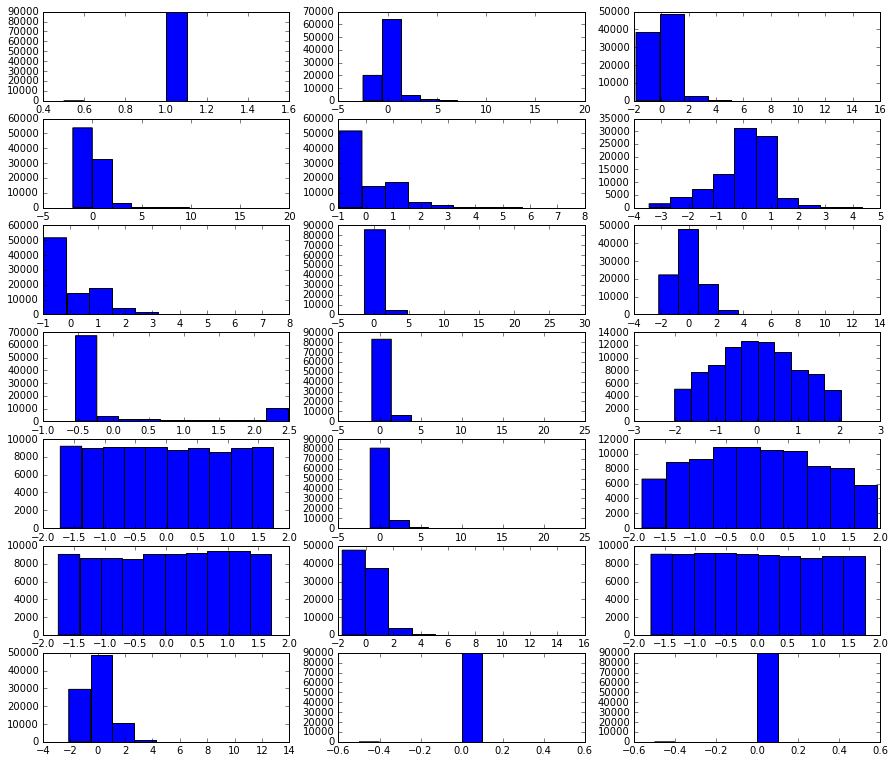
\includegraphics[width=\columnwidth]{img/features.png}
  \caption{Frequencies histograms of feature values of subset jet0 $m_h$}
  \vspace{-3mm}
  \label{hist}
\end{figure}


\subsection{Polynoms build}
We construct a polynom matrix of degree $d$ with our features matrix. The degree is chosen by 4-fold cross validation and is different for each of our eight datasets.

\subsection{Logistic Regression}
As we face a \emph{classification} problem, we choose to use a \emph{Logistic Regression} algorithm which shows good result as binary classifier. \cite{LRcourse} This choice leads to two problems to problems to take care:
\subsubsection{Rescale of the y's} 
As LR must be used for result values 0 or 1, we rescale $y in {-1, 1}$ to $y \in {0, 1}$. 

\subsubsection{Deal with overflow}
\emph{Double} value can handle number until $\sim 10^{304}$. This limit is reached with $exp(x)$ for $x \simeq 700$. To handle this problem, we use Taylor series of first order in both exponential and sigma functions. \cite{overflow}

For $s >> 1 \rightarrow 1+exp(s) \simeq exp(s)$ then 
$$
log(1+exp(s)) \simeq log(exp(s))=s.
$$
$$
exp(s)./(1+exp(s))\simeq 1
$$

For $0 < s << 1 \rightarrow exp(s)\simeq 1+s$ and then
$$
log(1+exp(s))\simeq log(2+s) \simeq log(2)+s/2
$$
$$
exp(s)./(1+exp(s)) \simeq 1/2+s/4.
$$


%========================
\section{Results}



%========================
\section{Discussion}


%========================
\section{Summary}

...


\bibliographystyle{IEEEtran}
\bibliography{literature}

\end{document}
